\documentclass{article}

\usepackage{graphicx}
\usepackage{tikz}
\usepackage{tikzsymbols}
\usetikzlibrary{calc,patterns,shapes.geometric}
\pagestyle{empty}
\usepackage[margin=0pt]{geometry}
\geometry{papersize={14in,12in}}

\def\centerarc[#1](#2)(#3:#4:#5){\draw[#1] ($(#2)+({#5*cos(#3)},{#5*sin(#3)})$) arc (#3:#4:#5);}

\begin{document}
	\begin{figure}
		\centering
		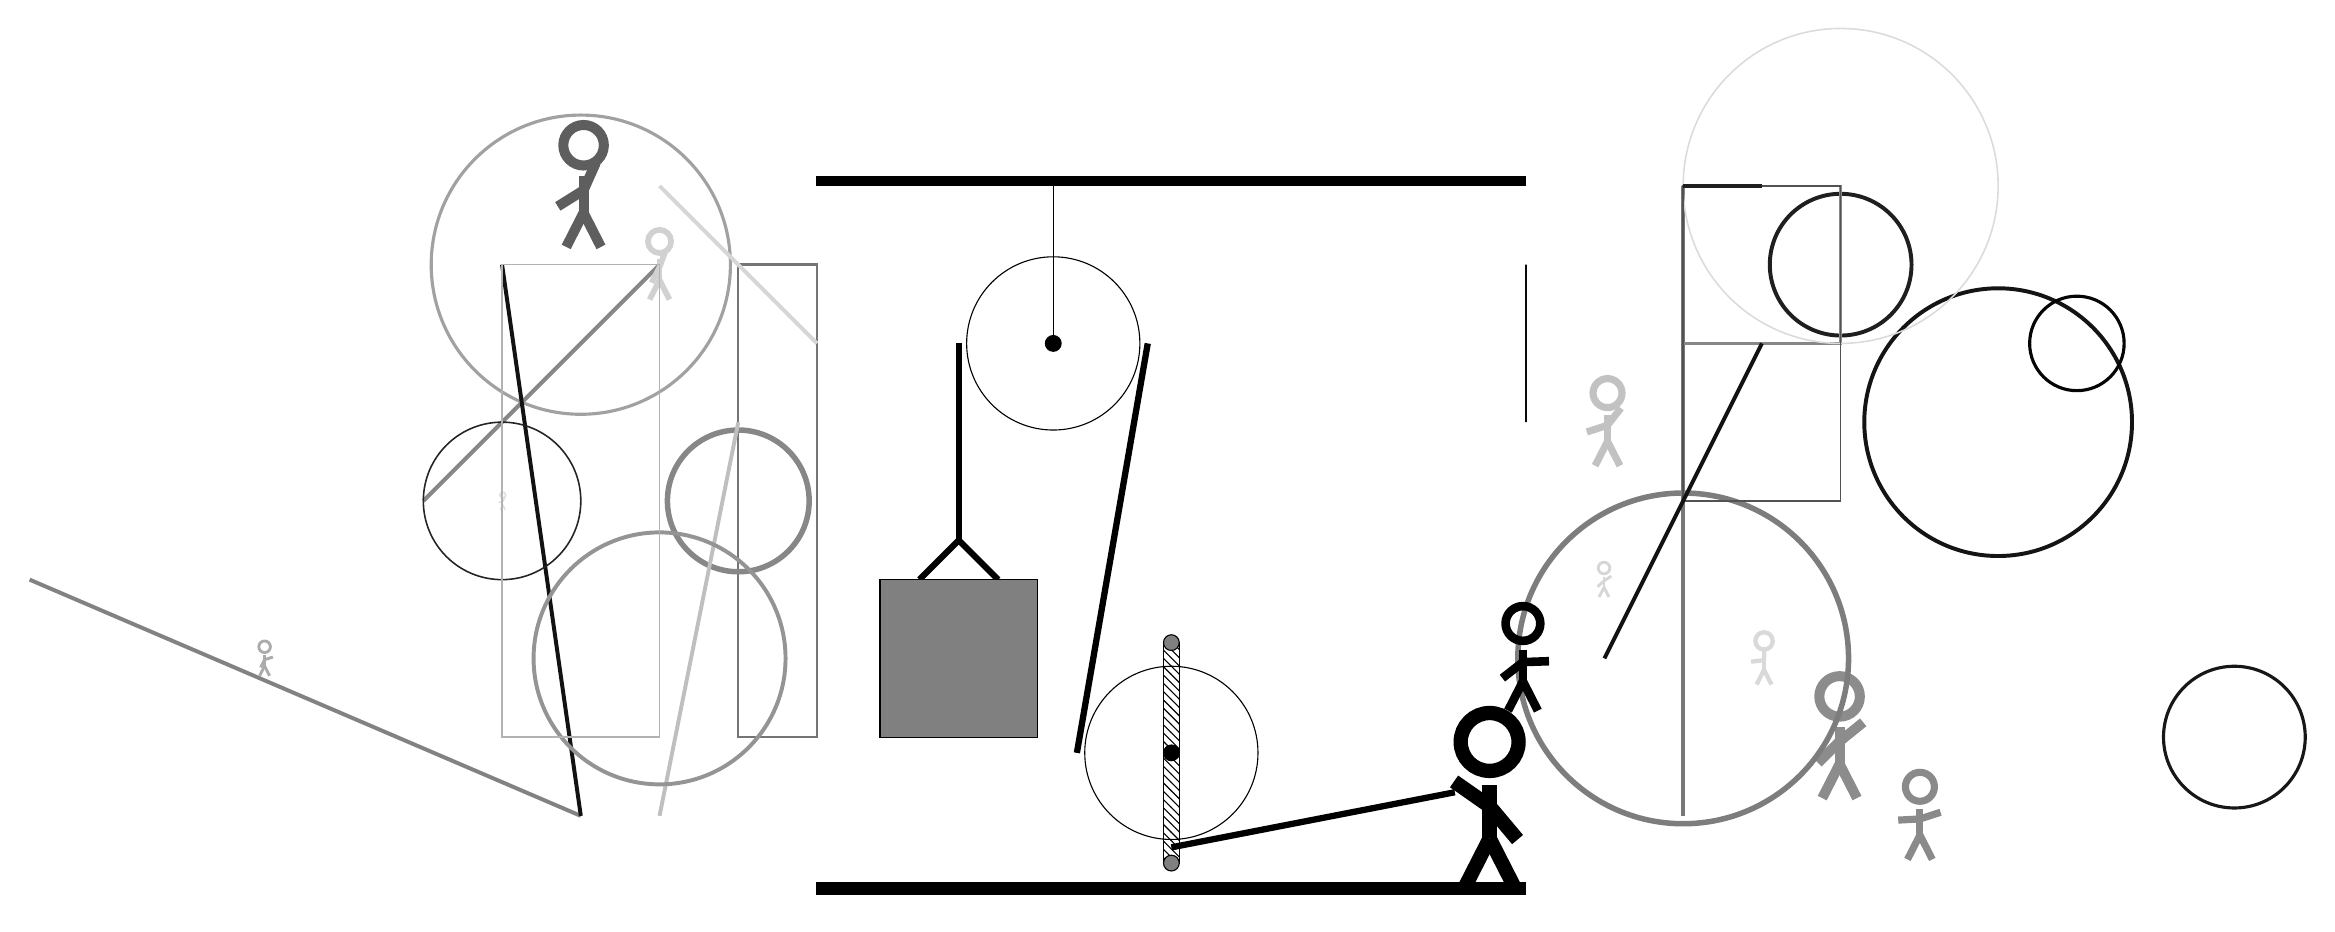
\begin{tikzpicture}
			%%%%% START %%%%%
			
			\draw[fill=black] (-2, 9) rectangle (7, 9.125);
			
			\draw (1, 7) circle (1.1);
			\draw[fill=black] (1, 7) circle (0.1);
			\draw (1, 9) -- (1, 7);
			
			\draw[fill=white](2.5, 1.8) circle (1.1);
			\draw[fill=black] (2.5, 1.8) circle (0.1);
			\draw[pattern=north west lines, pattern color=black] (2.4, 3.2) rectangle (2.6, 0.4);
			\draw[fill=black!50] (2.5, 3.2) circle (0.1);
			\draw[fill=black!50] (2.5, 0.4) circle (0.1);
			
			\draw[line width=0.8mm] (-0.7, 4.0) -- (-0.2, 4.5) -- (0.3, 4.0);
			\draw[fill=black!50] (-1.2, 4.0) rectangle (0.8, 2.0);
			
			\draw[line width=0.8mm] (-0.2, 7) -- (-0.2, 4.5);
			\centerarc[line width=0.8mm](1, 7)(0:180:1.2000000000000002);
			\draw[line width=0.8mm](2.2, 7) -- (1.3, 1.8);
			\centerarc[line width=0.8mm](2.5, 1.8)(180:270:1.2000000000000002);
			\draw[line width=0.8mm](2.5, 0.6) -- (6.1, 1.3);
			
			\node at (6.5, 1.2) {\Strichmaxerl[10][-35][-50]};
			
			\draw[line width=0.3mm, color=black!54] (-2, 2) rectangle (-3, 8);
			
			\draw [line width=0.7mm, color=black!47](-3, 5) circle (0.9);
			\draw[line width=0.5mm, color=black!49](-5, 1) -- (-12, 4);
			\node[line width=0.6mm, color=black!15] at (10, 3) {\Strichmaxerl[3][6][89]};
			\draw[line width=0.5mm, color=black!47](-7, 5) -- (-4, 8);
			
			\draw [line width=0.4mm, color=black!37](-5, 8) circle (1.9);
			\node[line width=0.5mm, color=black!45] at (11, 2) {\Strichmaxerl[7][45][39]};
			\draw [line width=0.5mm, color=black!88](11, 8) circle (0.9);
			\draw[line width=0.5mm, color=black!53] (9, 1) rectangle (9, 9);
			\draw[line width=0.5mm, color=black!93](-6, 8) -- (-5, 1);
			\draw [line width=0.5mm, color=black!92](13, 6) circle (1.7);
			\draw[line width=0.5mm, color=black!25](-4, 1) -- (-3, 6);
			\node[line width=0.6mm, color=black!33] at (-9, 3) {\Strichmaxerl[2][63][17]};
			
			\node[line width=0.6mm, color=black!24] at (8, 6) {\Strichmaxerl[5][18][52]};
			\draw [line width=0.4mm, color=black!98](14, 7) circle (0.6);
			\draw[line width=0.3mm, color=black!47] (9, 9) rectangle (11, 7);
			\draw[line width=0.2mm, color=black!96] (7, 6) rectangle (7, 8);
			\node[line width=0.4mm, color=black!46] at (12, 1) {\Strichmaxerl[5][3][18]};
			\draw [line width=0.2mm, color=black!86](-6, 5) circle (1.0);
			
			\draw[line width=0.5mm, color=black!16](-2, 7) -- (-4, 9);
			\draw [line width=0.4mm, color=black!91](16, 2) circle (0.9);
			
			\draw [line width=0.5mm, color=black!42](-4, 3) circle (1.6);
			\draw [line width=0.7mm, color=black!51](9, 3) circle (2.1);
			\node[line width=0.7mm, color=black!18] at (-4, 8) {\Strichmaxerl[4][63][70]};
			\draw [line width=0.2mm, color=black!14](11, 9) circle (2.0);
			
			\node[line width=0.2mm, color=black!13] at (-6, 5) {\Strichmaxerl[1][14][64]};
			
			\draw[line width=0.5mm, color=black!22](8, 1) -- (8, 1);
			\draw[line width=0.2mm, color=black!68] (9, 9) rectangle (11, 5);
			\node[line width=0.6mm, color=black!63] at (-5, 9) {\Strichmaxerl[7][32][66]};
			\node[line width=0.3mm, color=black!16] at (8, 4) {\Strichmaxerl[2][42][33]};
			\draw[line width=0.5mm, color=black!93](10, 7) -- (8, 3);
			
			\draw[line width=0.5mm, color=black!88](10, 9) -- (9, 9);
			\node[line width=0.3mm, color=black!100] at (7, 3) {\Strichmaxerl[6][38][2]};
			
			\draw[line width=0.2mm, color=black!30] (-4, 8) rectangle (-6, 2);
			
			
			\draw[fill=black] (-2, 0) rectangle (7, 0.15);
			
			%%%%% END %%%%%
		\end{tikzpicture}
	\end{figure}	
\end{document}